% !TEX root = Dokumentation.tex
\subsection{Projektunterstützung}
Während der Durchführung des Projekts soll der administrative Aufwand möglichst klein gehalten werden können. Weiter sollen alle Projektmitglieder gleichzeitig an der Software weiterentwickeln oder an der Dokumentation weiterschreiben können. Darum wird auf diverse Software-Produkte und Systeme zurückgegriffen, die sich in der Praxis bewährt haben.

\subsubsection{Software}
\begin{table}[H]
\begin{tabular}{|p{0.3\textwidth}|p{0.64\textwidth}|}\hline
	
Kommunikation	&	E-Mail, Whatsapp \\\hline
Dokumenterstellung & LaTeX\\\hline
Versionsverwaltungssoftware & Git \\\hline
Filehosting-Dienst & GitHub \\\hline
CAD-Software & NX\\\hline
Entwicklungsumgebung	& Eclipse, Kinetis Design Studio \\\hline

\end{tabular}\\
\end{table}
LaTeX ermöglicht es, die gesamte Dokumentation in mehrere Teildokumente zu unterteilen. All diese Dokumente sind in GitHub eingecheckt. Somit wird sichergestellt, dass mehrere Teammitglieder zur selben Zeit an der Dokumentation arbeiten können und dabei möglichst wenig Konflikte entstehen. Weiter wird auf dem selben Git-Repository auch der Quellcode der Software abgelegt. \\
\\
Um die Aufgabenverteilung festzuhalten wurde ein Scrum-Board erstellt. Darauf sind alle Team-Mitglieder aufgelistet. Zudem sind, wie bei Scrum üblich, die drei Zustände \glqq ToDo\grqq, \glqq Doing\grqq \ und \glqq Done\grqq \ definiert.
\begin{figure}[H]%Position festigen
\centering
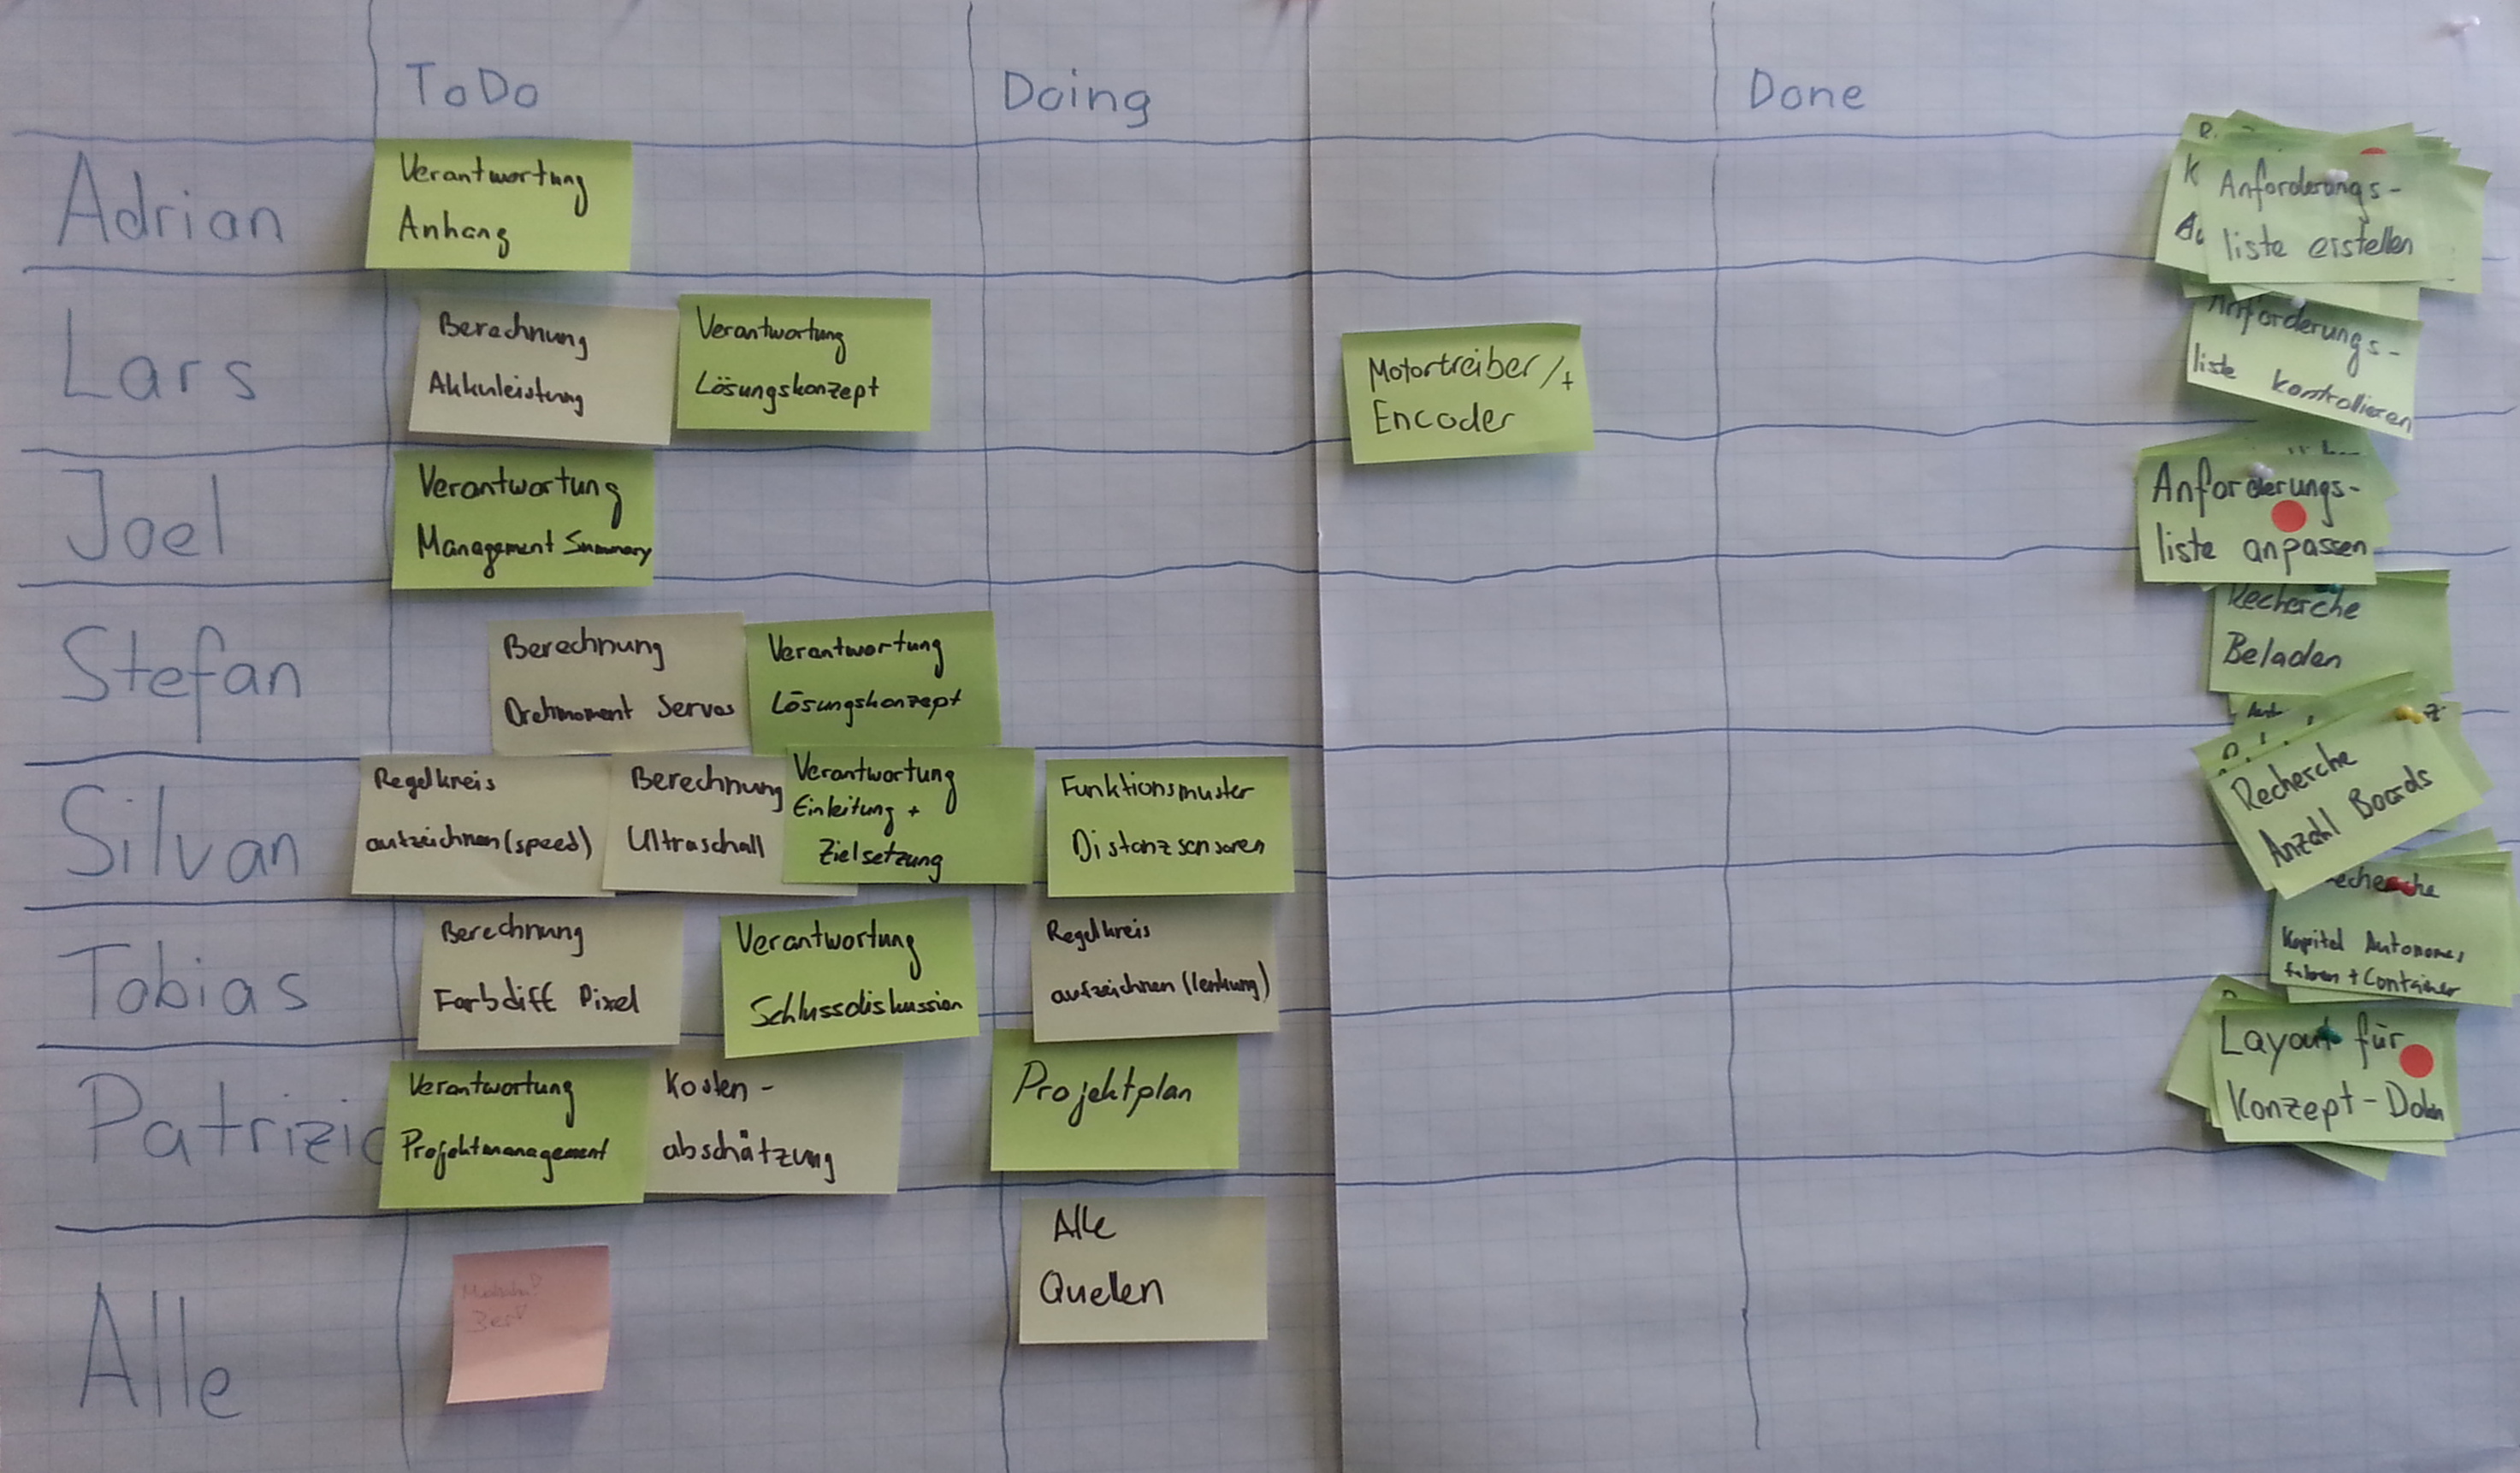
\includegraphics[width=0.8\textwidth]{04_Projektmanagement/fig/scrumBoard.jpg}
\caption{Scrum-Board}
\label{fig:scrumBoard}
\end{figure}